\section{Duality}
\subsection{Recap on subdifferential calculus}
Let $f:\mathbb{R}^n\to\mathbb{R}$ be a convex function. The subdifferential of $f$ at a point $x$ is defined as:
\begin{align*}
    \partial f : \R^n &\longrightarrow \Pc(\R^n)\\
    x &\longmapsto \partial f(x) = \set{g\in\R^n}{\forall y\in\R^n, \: f(y)\geq f(x)+g^\tp(y-x)}
\end{align*}
and any $g\in\partial f(x)$ is called a subgradient of $f$ at $x$. The subdifferential is a set-valued function, and it is always non-empty for convex functions. If $f$ is differentiable at $x$, then $\partial f(x) = \{\nabla f(x)\}$. The subdifferential is a generalization of the gradient for non-differentiable functions.

In the following, we derive formulae for the subdifferential of some common operations.

\begin{property}[Subdifferential of a scaled function]
    Let $f:\R^n\to\bar{\R}$ and $\alpha>0$. We define $h(x)=\alpha f(x)$. Then, for all $x\in\R^n$:
    \begin{equation*}
        \partial h(x) = \alpha\partial f(x)
    \end{equation*}
\end{property}

\begin{property}[Subdifferential of a composition with linear mapping]
    Let $f:\R^n\to\bar{\R}$ and $A\in\mathscr{M}_{n, d}(\R)$. We define $h(x)=f(Ax)$. Then, for all $x\in\R^n$:
    \begin{equation*}
        \partial h(x) = A^\tp\partial f(Ax)
    \end{equation*}
    when $\relint\dom h\neq\emptyset$.
\end{property}

\begin{property}[Subdifferential of a sum of functions]$ $\\
    Let $f_1, f_2:\R^n\to\bar{\R}$ and $(\relint\dom f_1)\cap (\relint\dom f_2)\neq\emptyset$. Then, for all $x\in\R^n$:
    \begin{equation*}
        \partial(f_1+f_2)(x) = \partial f_1(x) + \partial f_2(x)
    \end{equation*}
\end{property}

\begin{remark}
    \label{rm:constraint-qualification}
    The assumption $(\relint\dom f_1)\cap (\relint\dom f_2)\neq\emptyset$ is often referred to as a \emph{constraint qualification}. Such a constraint is necessary. Consider the following example: the function $\ind_{(0,0)}$ is the indicator function of the origin in $\R^2$. Its subdifferential at $(0, 0)$ is $\partial\ind_{(0,0)}((0, 0)) = \R^2$. Now, consider the following decomposition:
    \begin{equation*}
        \ind_{(0, 0)} = \frac{\ind_{B_1} + \ind_{B_1}}{2}
    \end{equation*}
    where $B_1 = B((-1, 0), 1)$ and $B_2 = B((1, 0), 1)$. The subdifferential of the sum is:
    \begin{equation*}
        \partial(\ind_{B_1}+\ind_{B_2})((0, 0)) = \set{(\alpha, 0)}{\alpha\in\R}
    \end{equation*}
    which is not equal to $\R^2$.
\end{remark}

\begin{remark}[About the composition rule]
    Let $S=\set{x\in\R^2}{x_1=x_2}$, and $f=\ind_S$. We define:
    \begin{equation*}
        A = \begin{bmatrix}
            0 & 0\\
            0 & 1
        \end{bmatrix}
    \end{equation*}
    We do have $f(Ax)=\ind_{(0, 0)}$, but the sets $\partial h(0)$ and $A^\tp\partial f(0)$ are not equal. This does not contradict the rule, as the constraint qualification is not satisfied ($\relint\dom f(A\cdot)=\emptyset$).
\end{remark}

\subsection{Fermat's rule}
\subsubsection{Definition}
\begin{theorem}[Fermat's rule]
    Let $f:\R^n\to\bar{R}$ be any function, and $x\in\R^n$. Then, $x$ is a minimizer of $f$ if and only if $0\in\partial f(x)$.
\end{theorem}
\begin{proof}
    A point $x$ minimizes $f$ if and only if:
    \begin{equation*}
        \forall y\in\R^n, \: f(y)\geq f(x) = f(x) + 0^\tp(y-x)
    \end{equation*}
    which by definition of the subdifferential is equivalent to $0\in\partial f(x)$.
\end{proof}
Note that Fermat's rule also holds for non-convex functions, even with local minimizers.

\begin{example}
    Consider the following function:
    \begin{figure}[H]
        \centering
        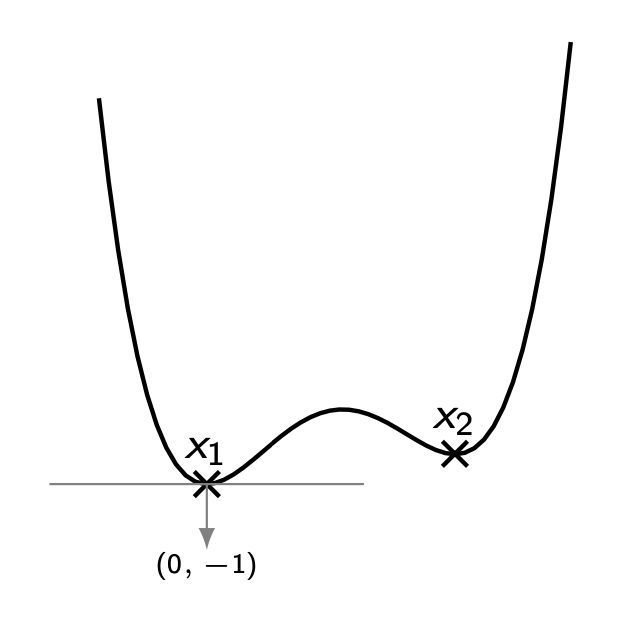
\includegraphics[width=.4\textwidth]{duality/fermat-rule.png}
    \end{figure}
    Then we have a global minimum at $x_1$:
    \begin{equation*}
        \partial f(x_1) = \{0\} \quad\text{and}\quad \nabla f(x_1)=0
    \end{equation*}
    and a local minimum at $x_2$:
    \begin{equation*}
        \partial f(x_2) = \emptyset \quad\text{and}\quad \nabla f(x_2)=0
    \end{equation*}
\end{example}

In general, it is difficult to check Fermat's rule directly; we need to resort on the structure of the problem. For instance, if the optimization problem involves several functions, such as:
\begin{equation*}
    \min_{x\in\R^n} f(x) + g(x)
\end{equation*}
then we can check the optimality of $x$ by verifying that $0\in\partial f(x) + \partial g(x)$. This also works under constraint qualifications (remember Remark \ref{rm:constraint-qualification}).

\subsubsection{Constraint qualifications}
Suppose that we want to solve the following optimization problem:
\begin{equation*}
    \min_x f(x) + \ind_{Q_1}(x) + \ind_{Q_2}(x)
\end{equation*}
For instance in $\R^2$, we might have $f((x_1, x_2))=x_2$, $Q_1=\set{x\in\R^2}{\norm{x-(1, 0)}\leq 1}$, and $Q_2=\set{x\in\R^2}{\norm{x+(1, 0)}\leq 1}$:
\begin{figure}[H]
    \centering
    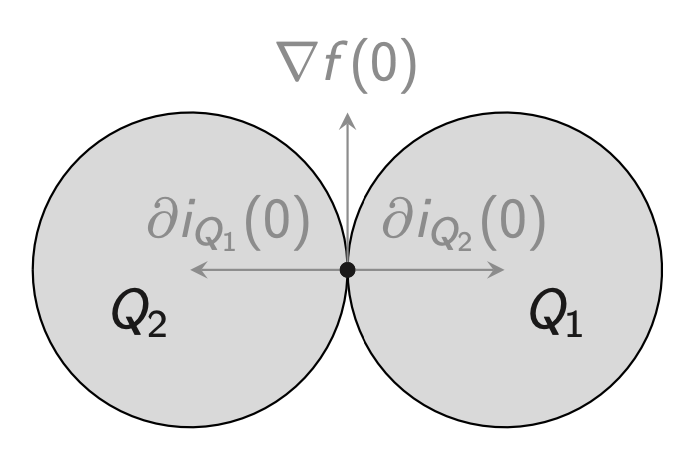
\includegraphics[width=.4\textwidth]{duality/q1-q2.png}
\end{figure}
There is no way to cancel the gradient using the sum of the subdifferentials, though $x=0$. This is because the constraint qualification is not satisfied. We need to directly check the subdifferential $\partial (f(x) + \ind_{Q_1} + \ind_{Q_2})$.

\subsubsection{Optimality conditions}
Let $f:\R^m\to\bar{\R}$, $g:\R^n\to\bar{\R}$ be closed, convex functions, and $A\in\mathscr{M}_{m, n}(\R)$. We study the following optimization problem:
\begin{equation}
    \label{eq:opt-condition}
    \min_x f(Ax)+g(x)
\end{equation}

\begin{theorem}[Slater's Constraint Qualification]
    \begin{equation}
        \tag{Slater-CQ}
        \exists \tilde{x}, \quad \tilde{x}\in(\relint\dom (f\circ A)) \cap(\relint\dom g)
    \end{equation}
\end{theorem}

Assuming Slater's constraint qualification, then $x^*\in\R^n$ is a solution to \autoref{eq:opt-condition} if and only if $x^*$ satisfies:
\begin{equation*}
    0\in A^\tp\partial f(Ax^*) + \partial g(x^*)
\end{equation*}
This optimality condition implies that for such $x^*$ there is some $\lambda\in\R^n$ such that:
\begin{equation*}
    \lambda\in A^\tp\partial f(Ax^*) \quad\text{and}\quad -\lambda\in\partial g(x^*)
\end{equation*}

\subsection{Fenchel-Legendre conjugation}
\subsubsection{Conjugate functions}
\begin{definition}[Conjugate function]
    The \emph{conjugate function} of $f:\R^n\to\R\cup\{+\infty\}$ is the function $f^*$ defined as:
    \begin{equation}
        \label{eq:conjugate}
        f^*(s):=\sup_x\left(s^\tp x-f(x)\right)
    \end{equation}
    This definition is implicit via the optimization problem above.
\end{definition}

The conjugate $f^*$ is the supremum of a family of affine functions. If we define $a_x(s)=s^\tp x-f(x)$ an affine function parametrized by $x$, then $f^*(s)=\sup_x a_x(s)$. 

The epigraph of $f^*$ is the intersection of the epigraphs of the $a_x$, which results in interesting properties for $f^*$.
\begin{figure}[H]
    \centering
    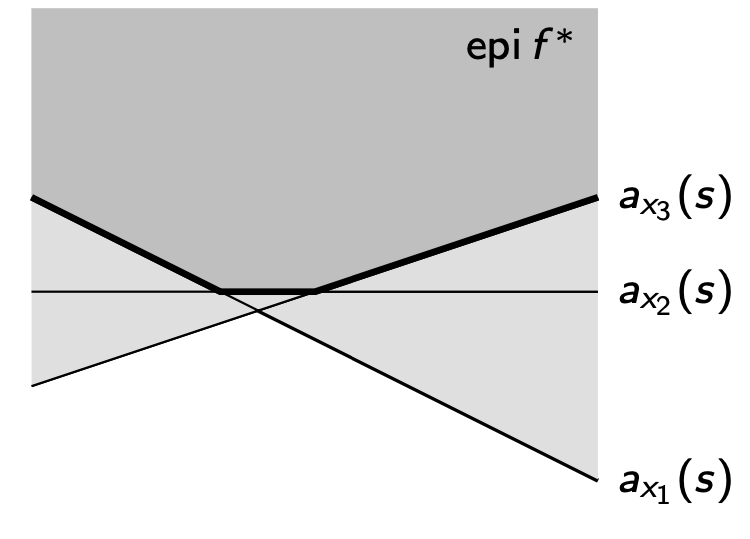
\includegraphics[width=.4\textwidth]{duality/epigraph-conjugate.png}
\end{figure}
\begin{property}$ $
    \begin{itemize}
        \item $f^*$ is convex, since its epigraph is the intersection of the convex halfspaces $\epi a_x$
        \item $f^*$ is closed, since its epigraph is the intersection of the closed halfspaces $\epi a_x$
        \item $f^*$ is proper if $\partial f(x)\neq\emptyset$ for some $x\in\R^n$
    \end{itemize}
    In the following, we will always assume this last hypothesis.
\end{property}

An interpretation of the conjugate $f^*(s)$ is that is defines an affine minorant of $f$ with slope $s$, where $-f^*(s)$ decides the constant offset to get support.
\begin{figure}[H]
    \centering
    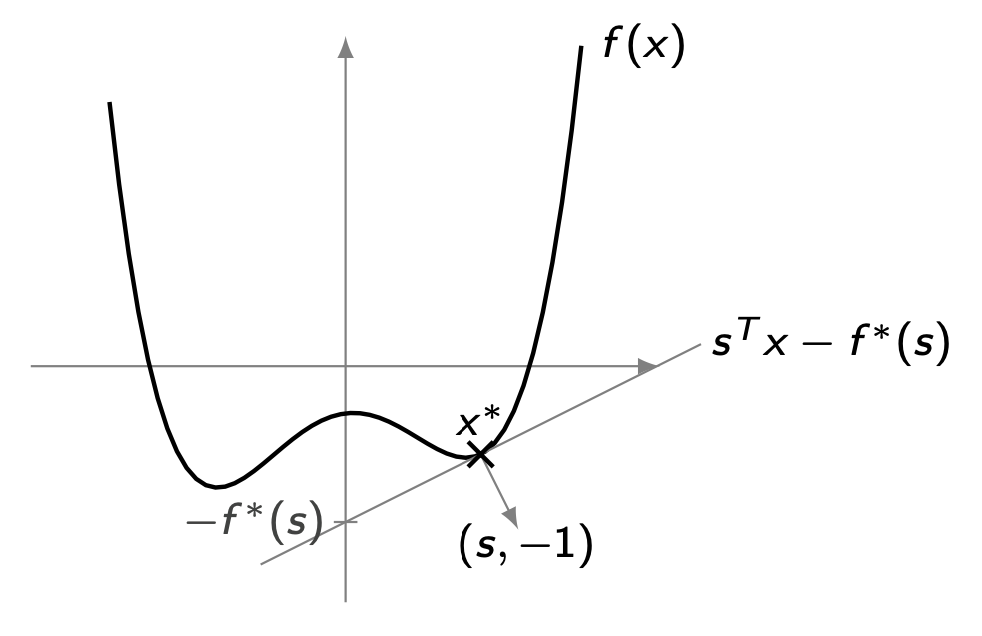
\includegraphics[width=.5\textwidth]{duality/affine-minorant.png}
\end{figure}
Formally:
\begin{align*}
    f^*(s) = \sup_x\left(s^\tp x-f(x)\right) 
    &\iff \forall x, \: f^s(s) \geq s^\tp x - f(x)\\
    &\iff \forall x, \: f(x) \geq s^\tp x - f^*(s)
\end{align*}
The maximizing argument $x^*$ gives support: $f(x^*)=s^\tp x^*-f^*(s)$. Furthermore, we have $f(x^*)=s^\tp x^*-f^*(s)$ if and only if $s\in\partial f(x^*)$.

\begin{property}
    The conjugate of $f$ and $\Conv f$\footnote{The \emph{convex closure} of $f$, noted $\Conv f$, is the function such that $\epi \Conv f=\Conv\epi f$.} are the same, that is:
    \begin{equation*}
        f^* = (\Conv f)^*
    \end{equation*}
    \begin{figure}[H]
        \centering
        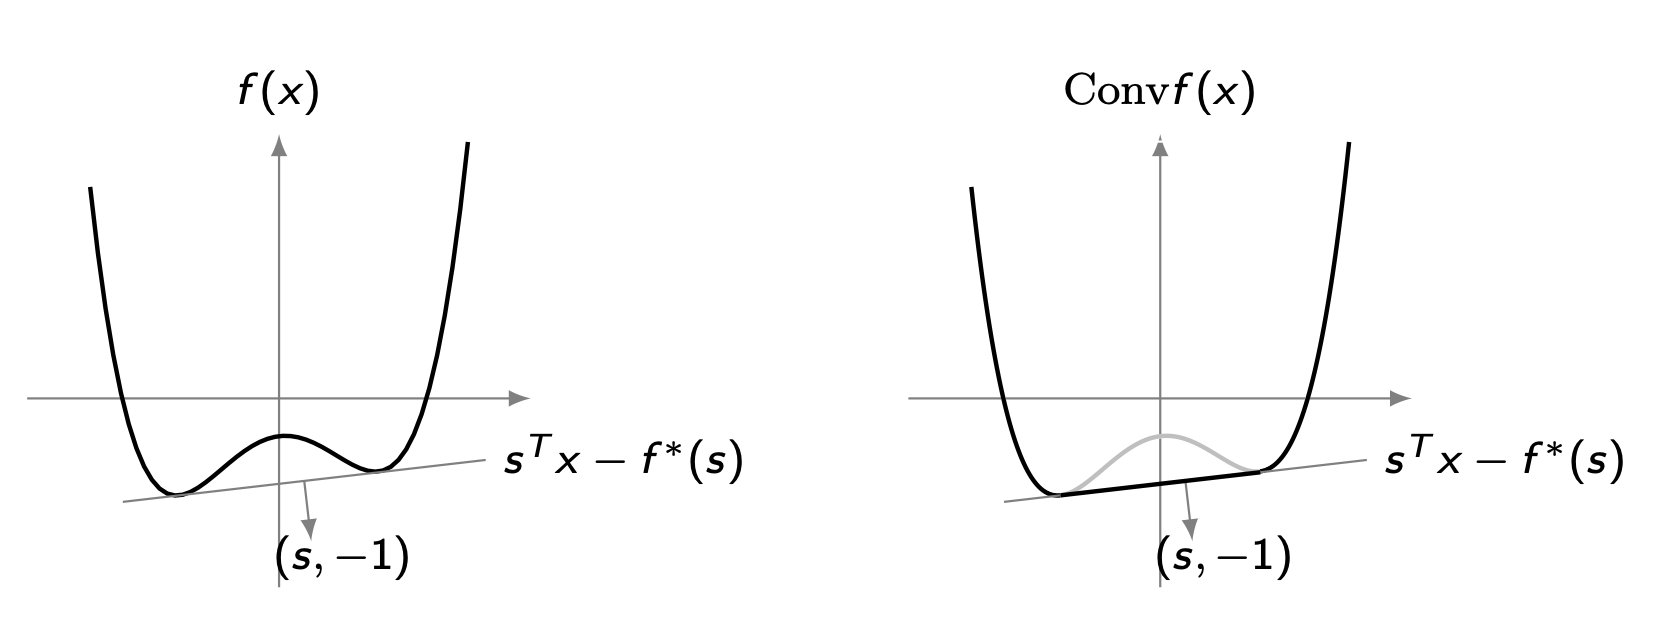
\includegraphics[width=.7\textwidth]{duality/conv-closure.png}
    \end{figure}
    Both functions have the same supporting affine functions, and both epigraphs have the same supporting hyperplanes.
\end{property}

\begin{example}[Conjugate of the absolute value]
    We aim at computing the conjugate of $f(x)=|x|$. By definition (\autoref{eq:conjugate}):
    \begin{equation*}
        f^*(s) = \sup_{x\in\R}\left(s^\tp x-f(x)\right)
    \end{equation*}
    If we choose $s<-1$, then $f^*(s)=+\infty$. For $-1\leq s\leq 1$, $f^*(s)=0$. For $s>1$, then $f^*(s)=+\infty$.
    \begin{figure}[H]
        \centering
        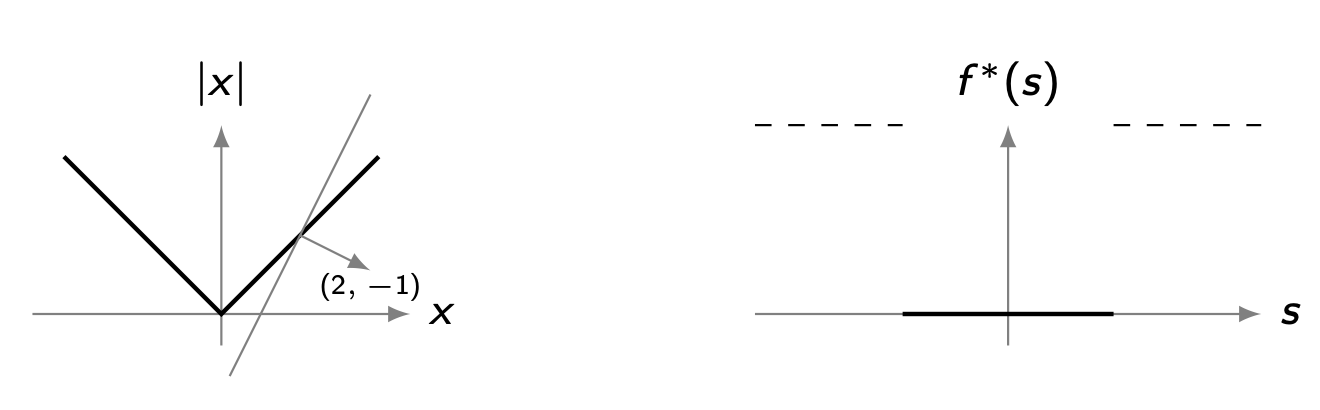
\includegraphics[width=.7\textwidth]{duality/conjugate-abs.png}
    \end{figure}
    Therefore, $f^*(s)=\ind_{[-1, 1]}(s)$.
\end{example}

\subsubsection{Biconjugate}
\begin{definition}[Biconjugate]
    The \emph{biconjugate} of $f:\R^n\to\R\cup\{+\infty\}$ is the function $f^{**}$ defined as:
    \begin{equation}
        \label{eq:biconjugate}
        f^{**}(x):=\sup_s\left(s^\tp x-f^*(s)\right)
    \end{equation}
    For every $x$, it is the largest value of all affine minorants of $f$.
    \begin{figure}[H]
        \centering
        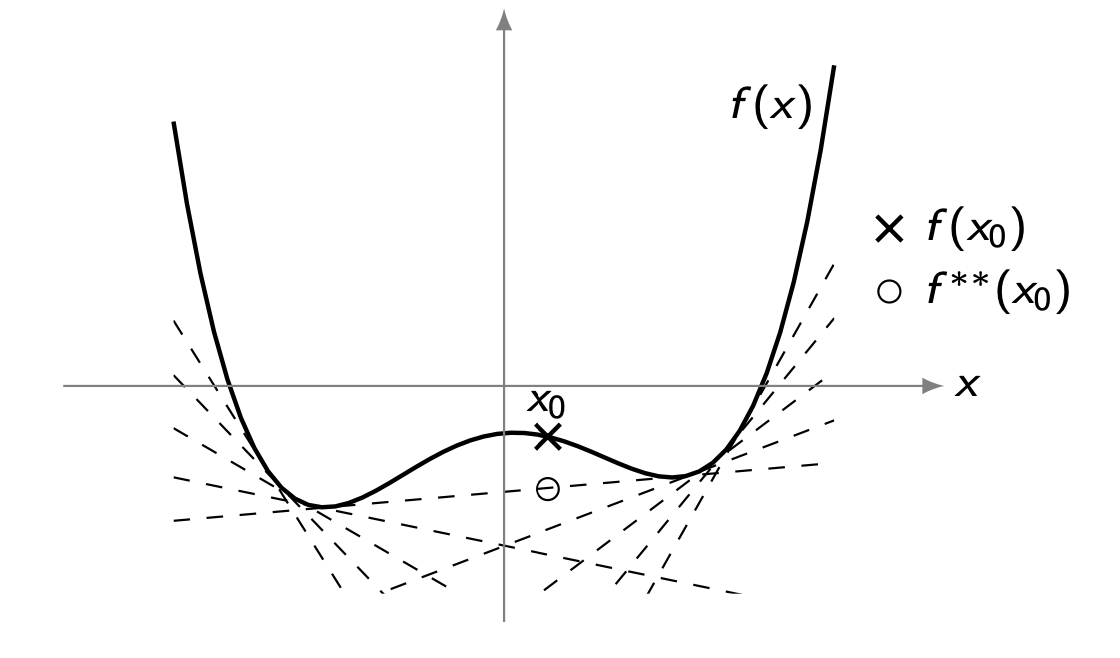
\includegraphics[width=.5\textwidth]{duality/biconjugate.png}
    \end{figure}
    Indeed, $x^\tp s-f^*(s)$ supports the affine minorant of $f$ with slope $s$. The biconjugate $f^{**}(x)$ picks the largest value over all these affine minorants evaluated at $x$.
\end{definition}

\begin{property}
    The biconjugate $f^{**}$ is the closed convex envelope of $f$:
    \begin{figure}[H]
        \centering
        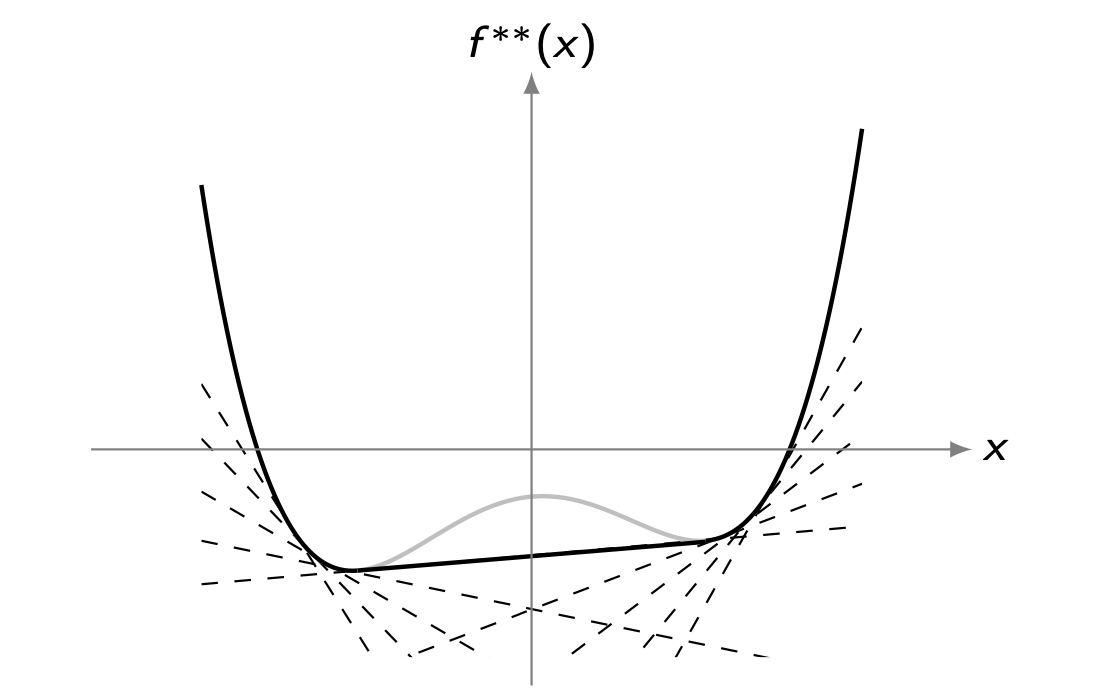
\includegraphics[width=.5\textwidth]{duality/biconjugate-envelope.png}
    \end{figure}
\end{property}
\begin{property}
    The following inequality always holds:
    \begin{equation*}
        f^**\leq f
    \end{equation*}
    with equality if and only if $f$ is closed and convex.
\end{property}